\chapter{Flow Past an Obstacle: Reproducing a Published Experiment}\label{ch09}
% generated by book/figures/ch09_texnumbers.py from ch09_numbers.json -- do not edit.  Each macro is math-mode material: write $\cnineForceTen$.
% macros are prefixed cnine to stay clear of the other chapters' names.
\newcommand{\cnineForceTc}{1.1\times10^{-6}}
\newcommand{\cnineForceLtOne}{4.0\times10^{-6}}
\newcommand{\cnineForceFive}{1.4\times10^{-4}}
\newcommand{\cnineForceTen}{2.2\times10^{-4}}
\newcommand{\cnineForceTwenty}{7.9\times10^{-3}}
\newcommand{\cnineForceThirty}{1.7\times10^{-2}}
\newcommand{\cnineForceForty}{1.7\times10^{-2}}
\newcommand{\cnineForceFifty}{1.6\times10^{-2}}
\newcommand{\cnineForceMax}{8.94}
\newcommand{\cnineForceMaxT}{47.8}
\newcommand{\cnineForceMaxTen}{5.45}
\newcommand{\cnineForceOverallPct}{0.19}
\newcommand{\cnineForceOverall}{1.68\times10^{-2}}
\newcommand{\cnineForceRelTen}{4\times10^{-5}}
\newcommand{\cnineForceRelTenTwo}{4.0\times10^{-5}}
\newcommand{\cnineForceRelTc}{6\times10^{-6}}
\newcommand{\cnineForceGrowth}{36}
\newcommand{\cninePlateauMean}{1.6\times10^{-2}}
\newcommand{\cninePlateauMin}{1.5\times10^{-2}}
\newcommand{\cninePlateauMax}{1.7\times10^{-2}}
\newcommand{\cnineZeroCross}{10.7}
\newcommand{\cninePlateauFracAtBirth}{82}
\newcommand{\cnineDragAtBirth}{7.1}
\newcommand{\cninedFatFourteen}{1.3\times10^{-3}}
\newcommand{\cninedFatTwenty}{8.0\times10^{-3}}
\newcommand{\cninedFatTwentyFour}{1.3\times10^{-2}}
\newcommand{\cninedFatTwentyEight}{1.6\times10^{-2}}
\newcommand{\cninedFatFifty}{1.5\times10^{-2}}
\newcommand{\cnineShiftTwenty}{0.12}
\newcommand{\cnineShiftThirty}{0.17}
\newcommand{\cnineShiftForty}{0.50}
\newcommand{\cnineShiftResTwenty}{4}
\newcommand{\cnineShiftResThirty}{26}
\newcommand{\cnineShiftResForty}{71}
\newcommand{\cnineLiftMax}{3.5\times10^{-4}}
\newcommand{\cnineLiftRatio}{4\times10^{-5}}
\newcommand{\cnineLiftRelMin}{0.4}
\newcommand{\cnineLiftRelMax}{3.6}
\newcommand{\cnineLiftZero}{3\times10^{-6}}
\newcommand{\cninePsiTen}{2.2\times10^{-4}}
\newcommand{\cninePsiGaugeTen}{2.1\times10^{-4}}
\newcommand{\cnineDensTen}{2.4\times10^{-4}}
\newcommand{\cnineNearShareTen}{11}
\newcommand{\cninePsiTwenty}{5.8\times10^{-4}}
\newcommand{\cninePsiGaugeTwenty}{4.8\times10^{-4}}
\newcommand{\cnineDensTwenty}{2.0\times10^{-4}}
\newcommand{\cnineNearShareTwenty}{10}
\newcommand{\cninePsiThirty}{1.3\times10^{-3}}
\newcommand{\cninePsiGaugeThirty}{1.0\times10^{-3}}
\newcommand{\cnineDensThirty}{2.0\times10^{-4}}
\newcommand{\cnineNearShareThirty}{39}
\newcommand{\cninePsiForty}{2.5\times10^{-3}}
\newcommand{\cninePsiGaugeForty}{1.9\times10^{-3}}
\newcommand{\cnineDensForty}{2.8\times10^{-4}}
\newcommand{\cnineNearShareForty}{72}
\newcommand{\cninePsiFifty}{4.1\times10^{-3}}
\newcommand{\cninePsiGaugeFifty}{3.3\times10^{-3}}
\newcommand{\cnineDensFifty}{4.0\times10^{-4}}
\newcommand{\cnineNearShareFifty}{80}
\newcommand{\cnineDensRmsMin}{2\times10^{-4}}
\newcommand{\cnineDensRmsMax}{4\times10^{-4}}
\newcommand{\cnineMaxDpsiFifty}{0.045}
\newcommand{\cnineMaxDnFifty}{0.0205}
\newcommand{\cnineGlobalPhaseFifty}{2.5\times10^{-3}}
\newcommand{\cninePaperVc}{0.18}
\newcommand{\cninePaperVth}{0.33}
\newcommand{\cninePaperRes}{2}
\newcommand{\cninePaperTLo}{2000}
\newcommand{\cninePaperTHi}{10000}
\newcommand{\cninePaperWx}{25}
\newcommand{\cninePaperWy}{20}
\newcommand{\cninePaperD}{3}
\newcommand{\cnineProdSteps}{5000}
\newcommand{\cnineProdWall}{2741}
\newcommand{\cnineProdWallMin}{46}
\newcommand{\cnineGammaCentre}{2.4\times10^{-6}}
\newcommand{\cnineGammaDisc}{1.7\times10^{-5}}
\newcommand{\cnineGammaOne}{1.39\times10^{-5}}
\newcommand{\cnineStopThr}{2\times10^{-5}}
\newcommand{\cnineEps}{5\times10^{-4}}
\newcommand{\cnineInitDouble}{2.8\times10^{-8}}
\newcommand{\cnineInitNoise}{4.1\times10^{-4}}
\newcommand{\cnineInitDiffPct}{10.0}
\newcommand{\cnineInitDiffN}{50\,077}
\newcommand{\cnineInitN}{500\,000}
\newcommand{\cnineInitRounded}{3\times10^{-18}}
\newcommand{\cnineOvershoot}{0.00275}
\newcommand{\cnineOvershootHalf}{0.001375}
\newcommand{\cnineSumV}{0.03025}
\newcommand{\cnineIntV}{0.0275}
\newcommand{\cnineRampOffset}{3.5\times10^{-3}}
\newcommand{\cnineRampOffsetHalf}{1.75\times10^{-3}}
\newcommand{\cnineSens}{1.27}
\newcommand{\cnineSensB}{1.2713}
\newcommand{\cnineSensA}{1.2709}
\newcommand{\cnineOwnTemporal}{3.3\times10^{-10}}
\newcommand{\cnineStageMin}{2.7\times10^{-3}}
\newcommand{\cnineStageMax}{3.5\times10^{-3}}
\newcommand{\cnineEqualCounts}{9}
\newcommand{\cnineCensusHeader}{5 & 10 & 15 & 20 & 25 & 30 & 35 & 40 & 45 & 50}
\newcommand{\cnineMatchThirty}{2}
\newcommand{\cnineMatchForty}{14}
\newcommand{\cnineMatchFiftyIdent}{9}
\newcommand{\cnineMatchFiftyClose}{1}
\newcommand{\cnineMatchTotalIdent}{25}
\newcommand{\cnineMatchTotal}{26}
\newcommand{\cnineWindN}{16}
\newcommand{\cnineWindDev}{3\times10^{-16}}
\newcommand{\cnineEdgeMax}{0.9993}
\newcommand{\cnineEdgeMargin}{0.07}
\newcommand{\cnineLoopDiffMax}{0.57}
\newcommand{\cnineLoopDiffThirty}{0.24}
\newcommand{\cnineMarginalInt}{0.951}
\newcommand{\cnineMarginalX}{82.5}
\newcommand{\cnineMarginalY}{4.0}
\newcommand{\cnineMarginalAbove}{5.7}
\newcommand{\cnineAsymZero}{5.7\times10^{-4}}
\newcommand{\cnineAsymRefFifty}{1.4\times10^{-4}}
\newcommand{\cnineAsymOursFifty}{1.8\times10^{-4}}
\newcommand{\cnineAsymOursFive}{3.9\times10^{-4}}
\newcommand{\cnineAsymRefTen}{2.2\times10^{-4}}
\newcommand{\cnineAsymOursTen}{3.5\times10^{-4}}
\newcommand{\cnineSupAreaOursFive}{192}
\newcommand{\cnineSupMOursFive}{1.85}
\newcommand{\cnineSupWidthOursFive}{16.5}
\newcommand{\cnineSupAreaOursTen}{254}
\newcommand{\cnineSupMOursTen}{2.22}
\newcommand{\cnineSupWidthOursTen}{20.5}
\newcommand{\cnineSupAreaOursFifteen}{321}
\newcommand{\cnineSupMOursFifteen}{2.84}
\newcommand{\cnineSupWidthOursFifteen}{23.5}
\newcommand{\cnineSupAreaOursTwenty}{378}
\newcommand{\cnineSupMOursTwenty}{5.38}
\newcommand{\cnineSupWidthOursTwenty}{26.5}
\newcommand{\cnineSupAreaRefTen}{253}
\newcommand{\cnineSupMRefTen}{2.21}
\newcommand{\cnineSupWidthRefTen}{20.5}
\newcommand{\cnineSupAreaRefTwenty}{380}
\newcommand{\cnineSupMRefTwenty}{5.42}
\newcommand{\cnineSupWidthRefTwenty}{26.5}
\newcommand{\cnineSupAreaOursTwentyP}{378.0}
\newcommand{\cnineSupAreaRefTwentyP}{379.5}
\newcommand{\cnineSupXminOursTwenty}{86.0}
\newcommand{\cnineSupXmaxOursTwenty}{102.5}
\newcommand{\cnineSupYhalfOursTwenty}{13}
\newcommand{\cnineSupXMmax}{89}
\newcommand{\cnineAxisNcentre}{0.25}
\newcommand{\cnineAxisUcentre}{0.70}
\newcommand{\cnineAxisMcentre}{1.40}
\newcommand{\cnineAxisJcentre}{0.17}
\newcommand{\cnineAxisJratio}{32}
\newcommand{\cnineAxisNmin}{0.086}
\newcommand{\cnineAxisSpeedMax}{1.58}
\newcommand{\cnineAxisMaxM}{5.4}
\newcommand{\cnineAxisXmin}{89}
\newcommand{\cnineAxisSupLo}{86.5}
\newcommand{\cnineAxisSupHi}{102.5}
\newcommand{\cnineUcFar}{0.876}
\newcommand{\cnineUcCentre}{0.409}
\newcommand{\cnineSqrtOneMinusV}{0.32}
\newcommand{\cnineBernB}{1.1513}
\newcommand{\cnineThrAreaOursFive}{201}
\newcommand{\cnineThrInOursFive}{84}
\newcommand{\cnineMachAreaNearOursFive}{192}
\newcommand{\cnineThrAreaOursTen}{289}
\newcommand{\cnineThrInOursTen}{88}
\newcommand{\cnineMachAreaNearOursTen}{254}
\newcommand{\cnineThrAreaOursFifteen}{379}
\newcommand{\cnineThrInOursFifteen}{95}
\newcommand{\cnineMachAreaNearOursFifteen}{321}
\newcommand{\cnineThrAreaOursTwenty}{450}
\newcommand{\cnineThrInOursTwenty}{99}
\newcommand{\cnineMachAreaNearOursTwenty}{378}
\newcommand{\cnineThrExcessOursTwenty}{19}
\newcommand{\cnineThrExcessOursFive}{5}
\newcommand{\cnineNBernCentre}{0.007}
\newcommand{\cnineNMeasCentre}{0.249}
\newcommand{\cnineBirthBefore}{24.2}
\newcommand{\cnineBirthAfter}{24.3}
\newcommand{\cnineBirthNmin}{9\times10^{-5}}
\newcommand{\cnineBirthNminAfter}{2.7\times10^{-4}}
\newcommand{\cnineBirthX}{86.75}
\newcommand{\cnineBirthY}{0.25}
\newcommand{\cnineBirthDist}{13.25}
\newcommand{\cnineBirthSep}{0.5}
\newcommand{\cnineBirthSepLate}{2.5}
\newcommand{\cnineBirthEdge}{0.998}
\newcommand{\cnineContRel}{1.2\times10^{-15}}
\newcommand{\cnineNminTwenty}{0.086}
\newcommand{\cnineNminTwentyThree}{9.1\times10^{-3}}
\newcommand{\cnineEdgeTwentyFour}{0.78}
\newcommand{\cnineEdgeTwentyFourTwo}{0.61}
\newcommand{\cnineBirthSupLo}{86.0}
\newcommand{\cnineBirthSupHi}{102.0}
\newcommand{\cnineBernCorr}{0.99999}
\newcommand{\cnineBernOneMinus}{7\times10^{-6}}
\newcommand{\cnineBernMaxDiff}{4.2\times10^{-3}}
\newcommand{\cnineBernRms}{0.12}
\newcommand{\cnineBernRspan}{0.6}
\newcommand{\cnineBernRlo}{-0.21}
\newcommand{\cnineBernRhi}{0.39}
\newcommand{\cnineBernQsmall}{0.028}
\newcommand{\cnineBernQmin}{-0.36}
\newcommand{\cnineBernQx}{88.5}
\newcommand{\cnineSonicS}{0.671}
\newcommand{\cnineVc}{0.144}
\newcommand{\cnineVzeroOverVc}{6.2}
\newcommand{\cnineJatVc}{0.017}
\newcommand{\cnineSatVc}{0.067}
\newcommand{\cnineVcApprox}{0.135}
\newcommand{\cnineCoreSound}{0.32}
\newcommand{\cnineCoreDensity}{0.1}
\newcommand{\cnineFreshMax}{5.40\times10^{-6}}
\newcommand{\cnineFreshRel}{8.1\times10^{-6}}
\newcommand{\cnineFreshCpu}{67}
\newcommand{\cnineFreshWall}{1169}
\newcommand{\cnineFreshLoadA}{12.7}
\newcommand{\cnineFreshLoadB}{24.9}
\newcommand{\cnineFreshPerStep}{0.67}
\newcommand{\cnineFreshLtOne}{4.0\times10^{-6}}
\newcommand{\cnineFreshTc}{1.13\times10^{-6}}
\newcommand{\cnineCensusRows}{%
reference detector, deposited file & 0 & 0 & 0 & 0 & 2 & 3 & 2 & 4 & 6 & 7 \\
same detector, our snapshots & 0 & 0 & 0 & 0 & 2 & 3 & 2 & 4 & 7 & 7 \\
exact census, ours & 0 & 0 & 0 & 0 & 2 & 2 & 4 & 14 & 10 & 10 \\
exact census, deposited fields & -- & 0 & -- & 0 & -- & 2 & -- & 14 & -- & 10 \\%
}
% macros \cnine... : every number below is the number of figures/ch09_numbers.json (generated by figures/ch09_texnumbers.py)

\section{A hole in the fluid}\label{ch09:hole}

At $t=24.2\,\tau$ the density of the fluid at one point of the axis, thirteen healing lengths downstream of the centre of the obstacle, is $\cnineBirthNmin$ of its bulk value. One tenth of a time unit later there are two vortices at that point, of opposite circulation, half a healing length apart. Nothing in the first twenty-four time units looked like dissipation: the flow was a smooth potential flow at $0.55$ of the speed of sound, the force on the obstacle had risen quietly to $\cnineDragAtBirth\,\mu/\xi$, and no vortex had been counted. These numbers do not come from a laboratory. They come from a numerical experiment, the example run that Junhwan Kwon and Yong-il Shin deposited with their paper on vortex shedding behind a penetrable obstacle in a two-dimensional superfluid \cite{KwonShin2026prr,KwonShin2026data}, and which we have reproduced, with an independent scheme, in the Rust engine of rusty-SUNDIALS. This chapter is about what that sentence means, what it cost, and what it leaves open.

Two remarks before anything else. First, \emph{experiment} means a computer experiment here. Laboratory experiments of this kind exist: a laser beam moved through a Bose--Einstein condensate gave an early measurement of a critical velocity \cite{Raman1999}, the periodic shedding of vortex dipoles from a moving penetrable obstacle \cite{Kwon2015PRA} and a von Kármán vortex street \cite{Kwon2016PRL}; we reproduce none of them. Second, nothing in this chapter reproduces or tests a measurement of Henri Godfrin, whose experiments are neutron-scattering measurements on helium (\cref{ch05,ch08}). The chapter belongs in a book dedicated to his work for another reason: it is where the book's three instruments are turned on somebody else's published result, and where the question ``do we agree?'' must be answered with numbers, the disagreements stated as plainly as the agreements, much as one checks an instrument against another laboratory's published number.

The three instruments appear in the following roles. The \emph{experiment} is the deposited run, the data we try to match: the wave function at six times, the force on the obstacle every tenth of a time unit, the output of the authors' vortex detector every five time units. The \emph{proof assistant} is used for what it is good at, the small exact statements on which a comparison silently leans: what Landau's criterion says about the uniform fluid, when a flow is locally supersonic, why the reference's velocity ramp is off by exactly $\cnineOvershoot\,\xi$, what makes a vortex count an integer. The \emph{solver} is \texttt{qf-pgpe::flow}, the obstacle-flow module of the Rust engine, which integrates the same equation as the reference with a different method, in a different precision, on a different machine.

\begin{figure}[t]\centering
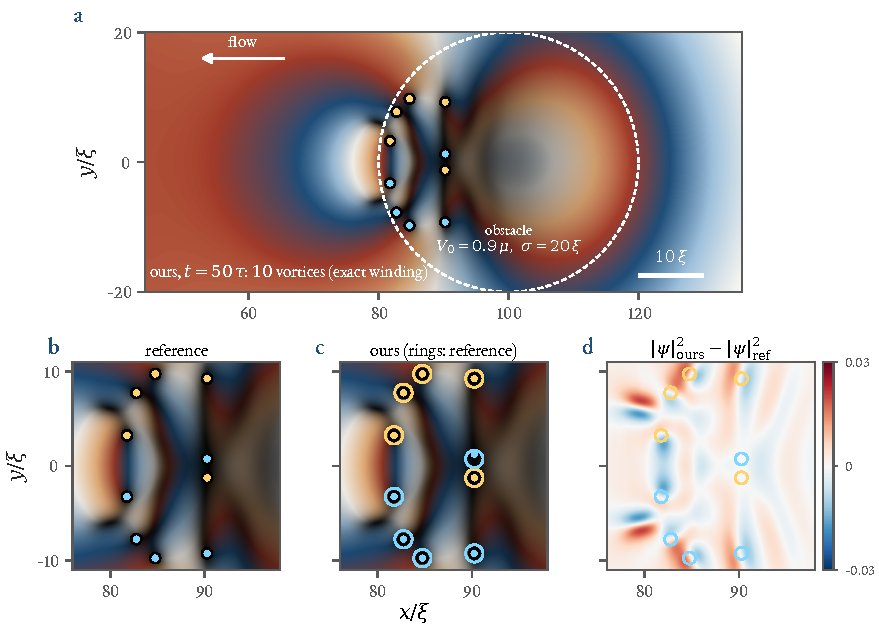
\includegraphics[width=\linewidth]{figures/ch09_wake.pdf}
\caption[The wake at $t=50\,\tau$]{The wake at $t=50\,\tau$. Hue is the phase of $\psi$, brightness its modulus (a hole in the fluid is black); the dots are plaquettes of non-zero winding (counter-clockwise gold, clockwise cyan; \cref{ch09:count}). \textbf{a}, our field; the dashed circle is the $1/\mathrm e^2$ radius of the obstacle and the fluid streams from right to left. \textbf{b}, \textbf{c}, the vortex region of the deposited field and of ours at eight times the grid resolution (spectral interpolation); the rings in \textbf{c} are the deposited vortices. \textbf{d}, $|\psi|^2_{\rm ours}-|\psi|^2_{\rm ref}$, at most $\cnineMaxDnFifty$ on the grid. Script \texttt{figures/ch09\_wake.py}.}\label{ch09:fig-wake}
\end{figure}

\Cref{ch09:fig-wake} is the picture to keep in mind. The broad lobes of colour are the phase of the potential flow around the obstacle. In panel \textbf{a} the ten dots are vortices, five pairs, each vortex the mirror image of an antivortex across the axis of the flow. The dark arcs through them are density troughs, lines on which the density is far below its bulk value. The deposited field and ours cannot be told apart at this magnification; panel \textbf{d} shows where they differ.

\section{The deposited run and the model}\label{ch09:model}

\paragraph{The archive.} The archive that accompanies the paper (Zenodo, version 1.0.0, 2026; code under the MIT licence, processed data to be reused with attribution under CC BY 4.0, as its README says \cite{KwonShin2026data}) holds the processed data behind the paper's summary figures (drag, lift and Strouhal number against a superfluid Reynolds number), the authors' GPU code (CuPy) with its configuration file, and one raw output case, for an obstacle of height $V_0=0.9\,\mu$ and width $\sigma=20\,\xi$ in a flow of $0.55$ times the speed of sound. For that case it gives the force on the obstacle every $0.1\,\tau$ and the output of the code's vortex detector every $5\,\tau$, both up to $t=100\,\tau$, and snapshots of the wave function every $10\,\tau$ from $t=0$ to $t=50\,\tau$. The README says what is not there: the full raw trajectories behind the paper's averages.

\paragraph{What we reproduce, and what we do not.} We reproduce the one raw case. We do not reproduce the paper's results, which rest on many parameter sets, each averaged over a window $\cninePaperTLo\le t\le\cninePaperTHi\,\tau$ \cite{KwonShin2026prr}, and on a post-processing (time-averaged irrotational flow, Mach-1 contour, effective diameter, Fourier analysis of the force) that we did not implement. Its central claims, a transition from periodic emission of vortex dipoles to the shedding of alternating same-sign vortex clusters at a superfluid Reynolds number $\mathrm{Re}_s\approx\cninePaperRes$ and the collapse of the Strouhal number and of the drag coefficient onto universal curves against $\mathrm{Re}_s$, are quoted as the authors' and not as ours. For the obstacle of the deposited case the paper reports a critical velocity $v_c\approx\cninePaperVc$ for dipole emission and a transition to cluster shedding at $v_{\rm th}\approx\cninePaperVth$ (in units of the speed of sound; every number of the paper quoted in this chapter is that of its arXiv version 1); the deposited run, at $0.55$, lies well above both.

\paragraph{The model.} In the units in which $\hbar=m=\mu=g=1$, the unit of length is the healing length $\xi=\hbar/\sqrt{m\mu}$, the unit of time is $\tau=\hbar/\mu$, the speed of sound of the uniform fluid is $c=\sqrt{\mu/m}=1$, the bulk density is $1$, and forces are measured in $\mu/\xi$. The deposited code integrates
\begin{equation}\label{ch09:eq-model}
\partial_t\psi \;=\; v(t)\,\partial_x\psi\;-\;\bigl(\mathrm i+\Gamma(x,y)\bigr)\Bigl[-\tfrac12\nabla^2+|\psi|^2-1\Bigr]\psi\;-\;\mathrm i\,V(x,y)\,\psi ,
\end{equation}
\begin{equation}\label{ch09:eq-pot}
V=V_0\exp\!\Bigl[-\frac{2\,\bigl((x-x_{\rm obs})^2+y^2\bigr)}{\sigma^2}\Bigr],\qquad v(t)=v_{\rm f}\,\min\!\bigl(t/t_{\rm acc},\,1\bigr),
\end{equation}
with $V_0=0.9$, $\sigma=20$, $x_{\rm obs}=100$, $v_{\rm f}=0.55$ and $t_{\rm acc}=0.1$, on a periodic grid of $1000\times500$ points of spacing $0.5\,\xi$ that covers $[-250,250)\times[-125,125)\,\xi$, with the time step $\Delta t=0.01\,\tau$. Read it term by term. Without $v$, $\Gamma$ and $V$ it is the Gross--Pitaevskii equation of \cref{ch03} with the chemical potential subtracted. The term $v\,\partial_x\psi$ moves to the frame of the obstacle: far away the fluid is at rest in the laboratory, the obstacle moves along $+x$ at speed $v$, and in the frame of the obstacle the fluid streams towards $-x$. The phase $\theta$ of $\psi$ is the laboratory phase, so the velocity relative to the obstacle is $\mathbf u=\nabla\theta-v\,\mathbf e_x$. The box is $500\,\xi\times250\,\xi$ and the obstacle sits at $x=100\,\xi$, so that the wake has $350\,\xi$ to run in. The damping function $\Gamma$ is $\cnineGammaCentre$ at the centre of the obstacle and at most $\cnineGammaDisc$ within its $1/\mathrm e^2$ radius, and rises to $\Gamma_0=0.1$ across layers that begin $50\,\xi$ and $40\,\xi$ from the edges of the box; in the layers the factor $(\mathrm i+\Gamma)$ turns the Hamiltonian evolution into a damped one, which absorbs the sound that the obstacle radiates before it can return through the periodic boundaries. The obstacle enters only through $-\mathrm iV\psi$: the deposited code treats $V$ as unitary and does not multiply it by the damping. The obstacle is \emph{penetrable} because $V_0<\mu$: at rest, the Thomas--Fermi density at its centre is $1-V_0=\cnineCoreDensity$ of the bulk, not zero.

Equation \eqref{ch09:eq-model} is what we recovered from the deposited code. The paper's own equation (1) agrees with it in its Hamiltonian part, and describes the damping layer (the ``fringe region'') with other numbers than the code does ($w_x=\cninePaperWx\,\xi$, $w_y=\cninePaperWy\,\xi$ and a transition scale $d=\cninePaperD\,\xi$, against layers of $50\,\xi$ and $40\,\xi$ and a scale of $15\,\xi$ in the code). We follow the code, because it is what produced the deposited run, and we have not tried to find out whether the two descriptions are equivalent in some convention.

\paragraph{Two schemes.} The deposited code advances \eqref{ch09:eq-model} by a splitting of Strang type: half a step of the linear part (kinetic term, moving-frame term, damping of the kinetic term) by a fourth-order Runge--Kutta method, a full step of the local part (nonlinearity, potential, constant offset) integrated exactly, and a second half step of the linear part, in single precision (\texttt{complex64}) on a GPU, with $\Delta t=0.01\,\tau$. Our scheme integrates the whole right-hand side of \eqref{ch09:eq-model} with one explicit fourth-order Runge--Kutta step, evaluates the derivatives spectrally, works in double precision, and uses the same $\Delta t$; we start it from the deposited field at $t=0$. The two computations therefore share the model and the initial data, and nothing else: not the scheme, not the precision, not the order of operations, not the machine. If they agree, the agreement is about the model and the data, not about a shared discretisation.

\paragraph{The force.} The force on the obstacle is the deposited code's
\begin{equation}\label{ch09:eq-force}
F_x=\iint \partial_xV\,|\psi|^2\,\mathrm dx\,\mathrm dy ,
\end{equation}
taken over the interior of the damping layers ($|x|<200\,\xi$, $|y|<85\,\xi$), with central differences for $\partial_xV$ and the trapezoidal rule, exactly as the code does. It is negative, the fluid pushing the obstacle along the flow, and we plot the drag $D=-F_x$. (The paper writes the force on the fluid, which is the opposite.) The lift $F_y$ is the same integral with $\partial_yV$.

\section{Why a subsonic flow can dissipate}\label{ch09:landau}

\paragraph{Landau's criterion.} An object of mass $M$ moves at speed $v$ through a fluid at rest. It can slow down only by creating an excitation of momentum $\hbar k$ and energy $\varepsilon(k)$, and conservation of energy and momentum then allows this only if
\begin{equation}\label{ch09:eq-landau}
v\;\ge\;\frac{\varepsilon(k)}{\hbar k}\quad\text{for some }k,\qquad\text{i.e.}\qquad v\;\ge\;v_{\rm L}:=\min_k\frac{\varepsilon(k)}{\hbar k}
\end{equation}
(for $M$ large against the excitation). Below $v_{\rm L}$ the object cannot dissipate energy into the fluid \cite{Landau1941}. The criterion needs one input, the spectrum $\varepsilon(k)$ of the elementary excitations of the fluid at rest.

\begin{godfrinbox}{The spectrum behind the criterion}
For superfluid $^4$He that spectrum is the dispersion curve of the Landau elementary excitations (phonon, maxon, roton) that Godfrin and his collaborators measured by inelastic neutron scattering at the ILL spectrometer IN5, and whose thermodynamic consequences they drew \cite{Godfrin2021}. In the review he wrote with Krotscheck, Landau's argument takes one paragraph \cite{GodfrinKrotscheck2022}: the creation of excitations by an object displaced in the fluid is impossible unless its velocity exceeds a critical value, and ``The linearity of the dispersion relation at low wave vectors is essential for this to happen''; in a Bose gas, whose dispersion is parabolic, the critical velocity is zero. These are statements about a curve that was \emph{measured}. The two lemmas below prove the inequalities behind them; they know nothing about helium, and nothing about the curve.
\end{godfrinbox}

\begin{leanbox}{HeliumKinematics}
\begin{lstlisting}[style=lean]
theorem landau_velocity_parabolic_zero {a : ℝ} (ha : 0 < a)
    {v : ℝ} (hv : 0 < v) :
    ∃ k : ℝ, 0 < k ∧ a * k ^ 2 / k < v := by
  refine ⟨v / (2 * a), by positivity, ?_⟩
  -- (proof abridged: three more lines)

theorem landau_velocity_ge_of_above_sound_line {ε : ℝ → ℝ}
    {c k : ℝ} (hk : 0 < k) (h : c * k ≤ ε k) : c ≤ ε k / k := by
  rw [le_div_iff₀ hk]; exact h
\end{lstlisting}
\end{leanbox}

In words: for a parabolic spectrum $\varepsilon=ak^2$ the ratio $\varepsilon/k=ak$ falls below any $v>0$ (take $k=v/2a$), so $v_{\rm L}=0$; a spectrum on or above the sound line $ck$ has $\varepsilon/k\ge c$ at every $k$. They are \Lthm{HeliumKinematics}{landau_velocity_parabolic_zero} and \Lthm{HeliumKinematics}{landau_velocity_ge_of_above_sound_line}, formalised from the review's paragraph, and they are theorems about real numbers, not about the experiment.

\paragraph{The uniform Gross--Pitaevskii fluid.} For the model \eqref{ch09:eq-model} the excitations of the uniform fluid are Bogoliubov's \cite{Bogoliubov1947}: in our units $\varepsilon(k)^2=\tfrac{k^2}2\bigl(\tfrac{k^2}2+2\bigr)$, that is $\varepsilon(k)=k\sqrt{1+k^2/4}$ (see \cref{ch05}). The following two statements are new Lean, written for this chapter (file \texttt{book/lean/Ch09\_FlowPast.lean}, namespace \texttt{QuantumFluids.FlowPast}; they are not part of the library). Compiled with Lean 4.34.0-rc2 and the matching Mathlib; no \texttt{sorry}; axioms \texttt{propext}, \texttt{Classical.choice}, \texttt{Quot.sound}.

\begin{leanbox}[title={Lean 4 \enspace FlowPast (new for this book)}]{Ch09\_FlowPast (new)}
\begin{lstlisting}[style=lean]
noncomputable def bogEps (k : ℝ) : ℝ := k * Real.sqrt (1 + k ^ 2 / 4)

theorem bogEps_ge_sound {k : ℝ} (hk : 0 ≤ k) : 1 * k ≤ bogEps k

theorem landau_uniform_gp :
    (∀ k : ℝ, 0 < k → 1 ≤ bogEps k / k) ∧
    (∀ δ : ℝ, 0 < δ → ∃ k : ℝ, 0 < k ∧ bogEps k / k < 1 + δ)
\end{lstlisting}
\end{leanbox}

The Landau velocity of the uniform Gross--Pitaevskii fluid is exactly the speed of sound (\Lthm{FlowPast}{landau_uniform_gp}): the ratio $\varepsilon/k$ never falls below $1$, and it comes within any $\delta$ of $1$, at $k=\sqrt{2\delta}$, where it equals $\sqrt{1+\delta/2}$ (proof abridged: the first clause is $\sqrt{1+k^2/4}\ge1$, the second is that identity and $\sqrt{1+\delta/2}<1+\delta$). The infimum is approached for $k\to0$ and never attained. Our obstacle moves at $0.55<1$. For the uniform fluid, \eqref{ch09:eq-landau} forbids every excitation, and the run nevertheless dissipates. (\Cref{ch05} proves the same statement for general $c$ and $m$: \Lthm{BogoliubovDispersion}{landau_velocity_eq}.)

\paragraph{The hypothesis that fails.} Landau's argument is about excitations of a fluid that is uniform, and an obstacle that disturbs it little. An obstacle of height $0.9\,\mu$ is not a small disturbance. At rest, the density in its core is a tenth of the bulk, and the local speed of sound there is $\sqrt{\cnineCoreDensity}=\cnineCoreSound$; a fluid forced through or around it must speed up. The criterion has to be applied locally, the local density fixing the local speed of sound. That is how Kwon and Shin read it: nucleation sets in when the flow becomes locally supersonic, $v(\mathbf r)>c_s(\mathbf r)=\sqrt{g\rho(\mathbf r)/m}$ (their equation (5), which they call the local Landau criterion), and they build their effective diameter, and with it their Reynolds number, on the Mach-1 contour of the time-averaged irrotational flow \cite{KwonShin2026prr}. The idea is older. Frisch, Pomeau and Rica found in the Gross--Pitaevskii model that vortex pairs are emitted behind an obstacle \cite{FrischPomeauRica1992}, and Josserand, Pomeau and Rica related the nucleation around a disk to the flow becoming locally supersonic at its edge \cite{JosserandPomeauRica1999}.

The following statements make the local criterion exact. They are again new Lean, in the same file.

\begin{leanbox}[title={Lean 4 \enspace FlowPast (new for this book)}]{Ch09\_FlowPast (new)}
\begin{lstlisting}[style=lean]
theorem supersonic_iff {n j : ℝ} (hn : 0 < n) (hj : 0 < j) :
    Real.sqrt n < j / n ↔ n ^ 3 < j ^ 2

theorem sonic_speed_threshold {n u V B : ℝ} (hB : n + u ^ 2 / 2 + V = B) :
    n < u ^ 2 ↔ 2 / 3 * (B - V) < u ^ 2

theorem bernoulli_min {s n : ℝ} (hs : 0 < s) (hn : 0 < n) :
    3 / 2 * s ≤ s ^ 3 / (2 * n ^ 2) + n

theorem barrier_height_bound {s n V : ℝ} (hs : 0 < s) (hn : 0 < n)
    (hB : s ^ 3 / (2 * n ^ 2) + n + V = 1 + s ^ 3 / 2) :
    V ≤ (1 - s) ^ 2 * (s + 2) / 2
\end{lstlisting}
\end{leanbox}

\emph{The first} (\Lthm{FlowPast}{supersonic_iff}) says that a flow of density $n$ and local flux $j=nu$ has $u>\sqrt n$, the local speed of sound, exactly when $n^3<j^2$, that is when the density is below the \emph{sonic density} $j^{2/3}$. It is algebra, and it is the form in which the data will be read below. \emph{The second} (\Lthm{FlowPast}{sonic_speed_threshold}) adds Bernoulli's relation $n+\tfrac12u^2+V=B$, the stationary hydrodynamic relation without quantum pressure, with $B=1+\tfrac12v^2$ for a fluid of density $1$ at speed $v$ far from the obstacle: the flow is locally supersonic exactly when $u^2>\tfrac23(B-V)$, a threshold on the speed that depends on the potential only. For $V=0$ it is the critical speed $u^2=\tfrac23+\tfrac13v^2$ that Josserand, Pomeau and Rica obtained for the flow past a disk; here it is $\cnineUcFar$ far from the obstacle, and $\cnineUcCentre$ at the centre of the obstacle, where $V=V_0=0.9$.

\emph{The last two} are a one-dimensional picture of the same mechanism. Take a steady flow in a channel, of flux $j$ conserved along the channel, and write $j^2=s^3$, so that $s$ is the sonic density. Bernoulli's function $j^2/(2n^2)+n$ is bounded below by $\tfrac32s$ (\Lthm{FlowPast}{bernoulli_min}), with equality only at the sonic point $n=s$ (\Lthm{FlowPast}{bernoulli_eq_iff}, in the file). The proof is a factorisation: $\frac{s^3}{2n^2}+n-\frac32s=\frac{(n-s)^2(2n+s)}{2n^2}\ge0$, the identity $2n^3-3sn^2+s^3=(n-s)^2(2n+s)$ being checked by \texttt{ring} (proof abridged). Consequently, if the fluid upstream has density $1$ and speed $j$, a steady state can exist at a point of the channel where the potential is $V$ only if $V\le V_c(s):=(1-s)^2(s+2)/2$ (\Lthm{FlowPast}{barrier_height_bound}): there is no steady flow over a barrier higher than that, the flow is \emph{choked}. For $j=0.55$ the sonic density is $s=\cnineSonicS$ and the ceiling is $V_c=\cnineVc$; the obstacle's $V_0=0.9$ is $\cnineVzeroOverVc$ times higher. As $j\to1$ (so $s\to1$) the ceiling $V_c$ tends to $0$: at the speed of sound any barrier chokes the flow, which is Landau's criterion again, seen from the other side.

\paragraph{What the one-dimensional theorem is not.} The ceiling $V_c$ reaches $V_0=0.9$ at $j=\cnineJatVc$, a factor of ten below the critical velocity $v_c\approx\cninePaperVc$ that Kwon and Shin find for the two-dimensional flow by testing for stationary solutions. The theorem does not predict that threshold, and LL-15, the programme's rule that an analogy is not a result, says why: it needs a flux conserved along the channel, and the flow has none. On the axis of the deposited run at $t=20\,\tau$ the flux at the centre of the obstacle is $j=\cnineAxisJcentre$, $\cnineAxisJratio\,\%$ of the upstream $0.55$: the stream lines have opened up. What survives is the structure of the picture, the sonic point as the minimum of Bernoulli's function and the supersonic region as the part of the flow beyond it. Kwon and Shin's own estimate of the supersonic region (their appendix A) uses Bernoulli and continuity in two dimensions to first order in $v/c$; they report that it overestimates the threshold and attribute the difference to the neglected quantum pressure, which they say is crucial in triggering shedding. The data below agree.

\paragraph{Reading the data.} \Cref{ch09:fig-mach} shows the field at $t=20\,\tau$, four time units before the first pair. The supersonic region is a single blob inside the obstacle, on its downstream half: on the axis it runs from $x=\cnineAxisSupLo$ to $\cnineAxisSupHi$ (the obstacle is centred at $100$), and it extends at most $\cnineSupYhalfOursTwenty\,\xi$ to either side. Its area is $\cnineSupAreaOursTwentyP\,\xi^2$ in our field and $\cnineSupAreaRefTwentyP\,\xi^2$ in the deposited one; the Mach number reaches $\cnineSupMOursTwenty$ and $\cnineSupMRefTwenty$ at $x=\cnineSupXMmax$, where the density is $\cnineAxisNmin$ and the flow runs at $\cnineAxisSpeedMax\,c$ relative to the obstacle; the two $M=1$ contours cannot be told apart. The blob existed earlier: its area is $\cnineSupAreaOursTen$ and $\cnineSupAreaRefTen\,\xi^2$ at $t=10$ and $\cnineSupAreaOursFive\,\xi^2$ at $t=5$ (maximal $M$: $\cnineSupMOursTen$, $\cnineSupMRefTen$ and $\cnineSupMOursFive$). The local criterion is thus satisfied for at least nineteen time units before the first pair appears: necessary, but nowhere near sufficient on a short time scale. The region has to deepen, the rarefaction behind it has to sharpen, and then a hole opens at its downstream end (the star in \cref{ch09:fig-mach}\textbf{a}).

\begin{figure}[t]\centering
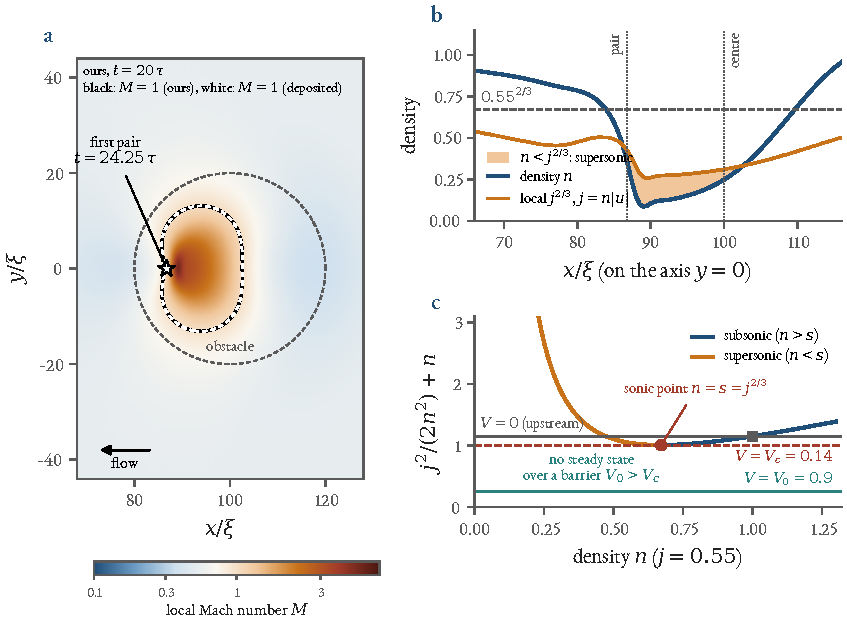
\includegraphics[width=\linewidth]{figures/ch09_mach.pdf}
\caption[The flow is locally supersonic long before the first vortex]{The flow is locally supersonic long before the first vortex. \textbf{a}, the local Mach number $M=|\nabla\theta-v\mathbf e_x|/\sqrt n$ of our field at $t=20\,\tau$; black, $M=1$ for our field; white dashes, $M=1$ for the deposited field; the star marks the first vortex pair, $t\approx24.25\,\tau$. \textbf{b}, the density and the local sonic density $j^{2/3}$, $j=n|\mathbf u|$, on the axis: $M>1$ exactly where $n<j^{2/3}$ (\lean{supersonic\_iff}). \textbf{c}, Bernoulli's function $j^2/(2n^2)+n$ of the channel at $j=0.55$ and the levels $1+j^2/2-V$ it must equal (\lean{bernoulli\_min}, \lean{barrier\_height\_bound}). Script \texttt{figures/ch09\_mach.py}.}\label{ch09:fig-mach}
\end{figure}

The threshold of \lean{sonic\_speed\_threshold} can be compared with this region without using the density. At $t=20$ the set where $|\mathbf u|^2>\tfrac23(B-V)$ has an area of $\cnineThrAreaOursTwenty\,\xi^2$ against the measured $\cnineMachAreaNearOursTwenty\,\xi^2$ and contains $\cnineThrInOursTwenty\,\%$ of it (at $t=5$, $10$, $15$: $\cnineThrInOursFive$, $\cnineThrInOursTen$, $\cnineThrInOursFifteen\,\%$), with an excess of area of $\cnineThrExcessOursFive\,\%$ at $t=5$ and $\cnineThrExcessOursTwenty\,\%$ at $t=20$. It predicts where the flow is supersonic well and what the density is poorly: Bernoulli's relation implies a density of $\cnineNBernCentre$ at the centre of the obstacle, where the measured one is $\cnineNMeasCentre$, because it needs a stationary flow (\cref{ch09:birth}).

\section{The reproduction}\label{ch09:repro}

\begin{keybox}[What ``reproduce'' means here]
Three things hide in the word. (i) The same input gives the same output, to rounding: the initial field is reproduced this way. (ii) A different scheme gives the same observables within a tolerance: for $t\le10$ the force agrees to $\cnineForceRelTen$ of its largest value, against a registered tolerance of $10^{-5}$ that was not met. (iii) The same events happen at the same times: the first vortex pair, the vortex counts. The fourth thing, reproducing the paper, is none of these and is not claimed.
\end{keybox}

\paragraph{What was run.} The flow solver is the module \texttt{flow} of the crate \texttt{qf-pgpe} (rusty-SUNDIALS, release v11.6.0; the Python extension \texttt{qf\_pgpe} does not expose it). It is driven by the example program \texttt{kwon\_shin}, which reads the deposited initial field and force, integrates, and writes the force every $0.1\,\tau$ and $\psi$ every $5\,\tau$. The production run to $t=50\,\tau$ took $\cnineProdSteps$ steps and $\cnineProdWall\,$s on the shared eight-core machine (load not recorded). Two excerpts of the source follow: the right-hand side \eqref{ch09:eq-model} (\texttt{ws.lap} is $\nabla^2\psi$, \texttt{ws.dxp} is $\partial_x\psi$, both spectral) and the velocities of the four stages.

\begin{rustbox}{qf-pgpe::flow, the source}
\begin{lstlisting}[style=rust]
// FlowSolver::rhs, last loop (excerpt)
for i in 0..psi.len() {
    let p = psi[i];
    let h = ws.lap[i] * (-0.5) + p * (p.norm_sqr() - 1.0);
    out[i] = ws.dxp[i] * v
        - (Complex64::new(self.gamma[i], 1.0)) * h
        - Complex64::new(0.0, self.potential[i]) * p;
}
// FlowSolver::step (excerpt): the velocity of the four stages
let (v1, v2, v3, v4) = match ramp {
    Ramp::StepEnd => {
        let v = self.velocity(t + dt);
        (v, v, v, v)
    }
    Ramp::StageTimes => (
        self.velocity(t),
        self.velocity(t + 0.5 * dt),
        self.velocity(t + 0.5 * dt),
        self.velocity(t + dt),
    ),
};
\end{lstlisting}
\end{rustbox}

\begin{rustbox}{qf-pgpe::flow, a fresh run}
A fresh run of the first time unit, made for this chapter (command, output and two rows of the force file as written; the path is shortened):
\begin{lstlisting}[style=plainmono]
$ kwon_shin --ref-dir .../20068724/extracted --t-end 1.0 --dt 0.01 --ramp step-end
step 0/100 t = 0.00 (1 s)
step 100/100 t = 1.00 (1169 s)
force_x: max |ours - reference| = 5.396e-6, relative to max |F| = 8.10e-6; wall 1169 s (100 steps)

t,force_x,force_ref,diff
0.300,-0.178067868131,-0.178068995476,1.127e-6
1.000,-0.665855021696,-0.665849626064,-5.396e-6
\end{lstlisting}
The hundred steps cost $\cnineFreshCpu\,$s of CPU time ($\cnineFreshPerStep\,$s per step, one thread) and $\cnineFreshWall\,$s of wall-clock time: the machine is shared (load average $\cnineFreshLoadA$ at the start, $\cnineFreshLoadB$ at the end), so the wall-clock figure measures the queue and not the code. The force column equals the first rows of the $\cnineProdSteps$-step run at the printed precision.
\end{rustbox}

\paragraph{The velocity ramp, and a convention that Lean can measure.} The deposited driver loops \texttt{for i in range(steps + 1): tt = i * dt; if i > 0: evolver.time\_evolv(tt)}, and \texttt{time\_evolv(tt)} uses $v(tt)$ in all of its stages. The step that takes the field from $(i-1)\Delta t$ to $i\Delta t$ therefore runs at the velocity of its \emph{end}. During the ramp ($0.1\,\tau$, ten steps) the obstacle moves relative to the fluid by $\sum_{i=1}^{10}v(i\Delta t)\Delta t=\cnineSumV$ instead of $\int_0^{0.1}v\,\mathrm dt=\cnineIntV$, an overshoot of $\cnineOvershoot\,\xi$. In general:

\begin{leanbox}[title={Lean 4 \enspace FlowPast (new for this book)}]{Ch09\_FlowPast (new)}
\begin{lstlisting}[style=lean]
theorem ramp_overshoot (a h : ℝ) (n : ℕ) :
    ∑ i ∈ range n, a * (((i : ℝ) + 1) * h) * h - a * ((n : ℝ) * h) ^ 2 / 2
      = a * h ^ 2 * n / 2
\end{lstlisting}
\end{leanbox}

Holding the velocity $at$ of a linear ramp at the end of each of $n$ steps of size $h$ overshoots the integral $a(nh)^2/2$ by exactly $ah^2n/2$ (\Lthm{FlowPast}{ramp_overshoot}; proof: induction on $n$ with one \texttt{nlinarith} for the step; abridged); with $a=v_{\rm f}/t_{\rm acc}=5.5$, $h=0.01$ and $n=10$ this is the $\cnineOvershoot$ above. The solver measures the same thing. With the velocity read at the stage times the force differs from the deposited one by $\cnineRampOffset$ at $t=0.1\,\tau$ (between $\cnineStageMin$ and $\cnineStageMax$ up to $t=5$); with the reference's reading it differs by $\cnineForceTc$ for $t\le0.3$. Halving $\Delta t$ halves the overshoot, to $\cnineOvershootHalf\,\xi$, and the offset goes down to $\cnineRampOffsetHalf$; the offsets are the same multiple of the displacement that separates the two runs, $\cnineSensA$ and $\cnineSensB\;\mu/\xi^2$. The convention is a displacement of the obstacle relative to the fluid by the amount that the theorem computes. It also means that halving $\Delta t$ with the reference's convention is not a convergence test, since the convention depends on $\Delta t$. Our own temporal error, with the stage-time reading, is $\cnineOwnTemporal$ in the force over $t\le5$ ($\Delta t=0.01$ against $0.005$), negligible against every other number in this chapter.

The library module \texttt{HeliumKinematics} does the same kind of small job for the analysis of the neutron time-of-flight data of the 2021 paper: it proves that two printed energy formulas (its equations 12 and 13) are one formula once the flight distance and the incident energy are written through the incident velocity (\Lthm{HeliumKinematics}{tof_eq12_eq_eq13}) and that rescaling the energy calibration cannot change whether one measured energy exceeds twice another (\Lthm{HeliumKinematics}{plateau_excess_calibration_invariant}): what a convention can and cannot move, settled once. The resemblance is one of method; it says nothing about neutron scattering.

\paragraph{The initial field.} The deposited initial field is itself a finding. The code prepares it by imaginary-time propagation from the Thomas--Fermi field, stopping when the integral $\gamma$ of $|\psi_{\rm new}-\psi_{\rm old}|^2$ falls below $\epsilon\,\delta\tau$, with the deposited tolerance $\epsilon=\cnineEps$ and $\delta\tau=0.04$, that is below $\cnineStopThr$. We re-derived the field in a few lines of numpy from the code's operators. After \emph{one} step $\gamma=\cnineGammaOne<\cnineStopThr$: the loop stops at its first iteration. The stored $\psi(t=0)$ is therefore the Thomas--Fermi field after one imaginary-time step plus the seeded noise ($10^{-4}$ times integers in $[-5,5)$ for the real and the imaginary part, relative size $\cnineInitNoise$), not a relaxed stationary state of the obstacle problem. Our array, rounded to \texttt{complex64}, equals the stored one bit for bit in $90\,\%$ of its $\cnineInitN$ elements; the other $\cnineInitDiffN$ (those where the noise has a zero imaginary part) differ by floating-point residues below $2\times10^{-16}$. In double precision the distance is $\cnineInitDouble$, the rounding of \texttt{complex64}. This is a statement about the deposited data and not a criticism of the paper, which describes the initial state as relaxed to the ground state and measures its observables long after any relaxation of the initial field; but anyone who uses the deposited $\psi(0)$ as a ground state should know that the early force contains that relaxation.

\paragraph{Results.} \Cref{ch09:tab-repro} collects the comparisons, \cref{ch09:fig-force} shows the force. All numbers are computed by \texttt{figures/ch09\_numbers.py} from the deposited files and our snapshots.

\begin{table}[t]\centering\small
\begin{tabular}{@{}p{0.31\linewidth}p{0.63\linewidth}@{}}\toprule
quantity & ours against the deposited run\\\midrule
initial field & bit for bit after rounding to \texttt{complex64} in $90\,\%$ of the elements; $\cnineInitDouble$ in double precision\\
force $\max|\Delta F|$, $t\le0.3$; $<1$; $\le5$; $\le10$ & $\cnineForceTc$; $\cnineForceLtOne$; $\cnineForceFive$; $\cnineForceTen$ ($\cnineForceRelTenTwo$ of the largest force, $\cnineForceMaxTen$, of that window)\\
force, windows $10$--$20$, $20$--$30$, $30$--$40$, $40$--$50$ & $\cnineForceTwenty$; $\cnineForceThirty$; $\cnineForceForty$; $\cnineForceFifty$ ($\cnineForceOverallPct\,\%$ of the largest force, $\cnineForceMax$)\\
$\psi$ at $t=10,20,30,40,50$ (relative $L^2$) & $\cninePsiTen$, $\cninePsiTwenty$, $\cninePsiThirty$, $\cninePsiForty$, $\cninePsiFifty$; after removing a global phase $\cninePsiGaugeTen$, $\cninePsiGaugeTwenty$, $\cninePsiGaugeThirty$, $\cninePsiGaugeForty$, $\cninePsiGaugeFifty$\\
density $|\psi|^2$ (relative $L^2$) & $\cnineDensTen$, $\cnineDensTwenty$, $\cnineDensThirty$, $\cnineDensForty$, $\cnineDensFifty$\\
lift $F_y$ at the snapshot times & within $\cnineLiftRelMin$--$\cnineLiftRelMax\,\%$ of the deposited values ($|F_y|\le\cnineLiftMax$)\\
vortex census, $t=30,40,50$ & $\cnineMatchTotalIdent$ of $\cnineMatchTotal$ vortices on the same plaquette, one within one cell\\
count of the deposited detector & equal at $\cnineEqualCounts$ of $10$ times\\
supersonic region, $t=20$ & area $\cnineSupAreaOursTwentyP$ against $\cnineSupAreaRefTwentyP\,\xi^2$; $M_{\max}$ $\cnineSupMOursTwenty$ against $\cnineSupMRefTwenty$\\
own temporal error & $\cnineOwnTemporal$ in the force, $t\le5$\\\bottomrule
\end{tabular}
\caption{Our Rust run against the deposited run. Every row is recomputed here from the raw files. The rows on the initial field, the force, $\psi$, the density and the detector's counts repeat numbers of the programme's earlier record (\texttt{docs/designs/PGPE\_EXTERNAL\_REPRODUCTION.md}); the gauge-fixed distances, the lift, the census and the supersonic region are new.}\label{ch09:tab-repro}
\end{table}

\begin{figure}[t]\centering
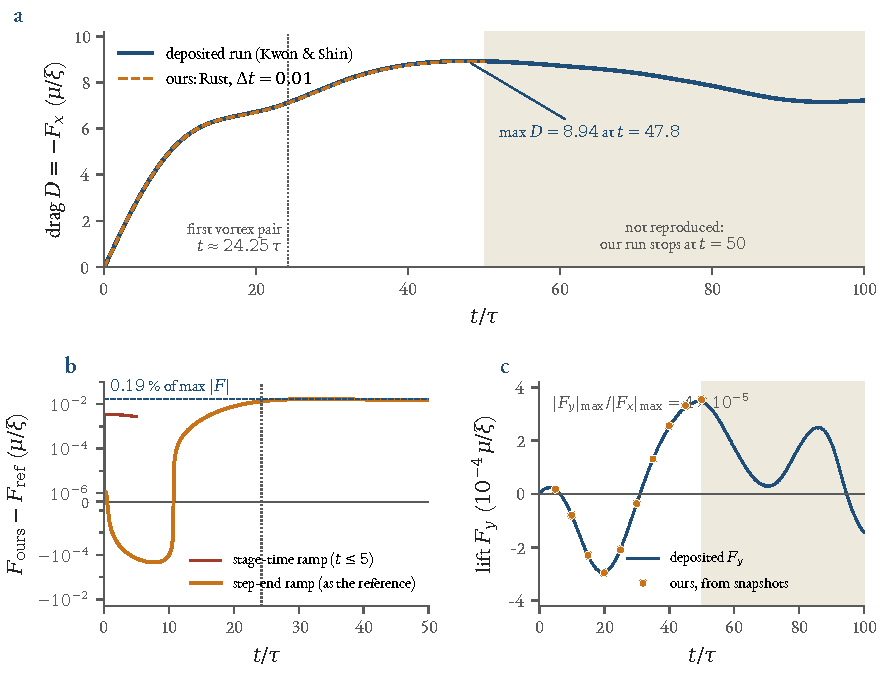
\includegraphics[width=\linewidth]{figures/ch09_force.pdf}
\caption[The force on the obstacle]{The force on the obstacle. \textbf{a}, the drag $D=-F_x$ of the deposited run to $t=100\,\tau$ (blue) and of our Rust run to $t=50\,\tau$ (orange dashes). \textbf{b}, the difference $F_{\rm ours}-F_{\rm ref}$ on a symmetric logarithmic axis, with the reference's step-end reading of the velocity (orange) and with the stage-time reading up to $t=5$ (red); the dotted line marks the first vortex pair. \textbf{c}, the lift $F_y$ of the deposited run and ours at the snapshot times. Script \texttt{figures/ch09\_force.py}.}\label{ch09:fig-force}
\end{figure}

Three things stand out. The agreement is at the level of $10^{-6}$ for the first time unit and $10^{-4}$ for the first ten, which is what two accurate integrators of the same equation should give, and it was reached with a scheme, a precision and a machine that have nothing in common with the reference's. Second, the tolerance that the programme had registered for this item of its plan, a relative force agreement of $10^{-5}$ for $t\le10$, is not met: it is $\cnineForceRelTen$ of the largest force of that window (it is $\cnineForceRelTc$ for $t\le0.3$). The criterion was set before the reference's velocity convention was known, and the plan keeps it as failed. No criterion had been registered for $t>10$; the second half of the table is reported as found. Third, from $t\approx\cnineZeroCross$ the force difference changes sign, grows, and levels off at about $\cninePlateauMean$, $\cnineForceOverallPct\,\%$ of the largest force, for $t\ge26$. \Cref{ch09:gaps} comes back to it, because the first reading of that growth that the programme gave is not supported by the data.

\section{Counting vortices}\label{ch09:count}

\paragraph{What a count is.} A vortex is a point where the wave function vanishes and its phase winds by $2\pi$; a grid sees only $\psi$ at its points. The standard way out, used by many vortex-finding codes, is to add up the \emph{principal differences} of the phase around each plaquette (an elementary square of four grid points) and to divide by $2\pi$. The proof assistant has something exact to say about that procedure: it rests on a statement that is true for a reason, and it fails for a reason.

\begin{leanbox}{VortexWinding}
\begin{lstlisting}[style=lean]
noncomputable def pdiff (a b : ℝ) : ℝ := toIocMod two_pi_pos (-π) (b - a)

theorem loop_sum_eq_mul (θ : ℕ → ℝ) (n : ℕ) (hclosed : θ n = θ 0) :
    ∃ m : ℤ, ∑ i ∈ Finset.range n, pdiff (θ i) (θ (i + 1))
      = (m : ℝ) * (2 * π) := by
  -- (proof abridged: pdiff = (b - a) - integer * 2π, then the sum telescopes)

theorem pdiff_add_rev_eq_two_pi_iff (a b : ℝ) :
    pdiff a b + pdiff b a = 2 * π ↔ (pdiff a b = π ∧ pdiff b a = π)
\end{lstlisting}
\end{leanbox}

The first theorem, \Lthm{VortexWinding}{loop_sum_eq_mul}, says that for \emph{any} closed list of phases $\theta_0,\dots,\theta_n=\theta_0$ the sum of the principal differences along the loop is an integer multiple of $2\pi$ (here \texttt{pdiff a b} is the representative of $b-a$ in $(-\pi,\pi]$): that a computed winding number is an integer is a theorem and not a numerical accident. The second says exactly when an edge fails to cancel. Walked in both directions an edge gives $0$, unless both principal differences equal $\pi$, which add up to $2\pi$; at that single value the cancellation between the two plaquettes that share the edge breaks, and a spurious winding can appear. With no edge at $\pi$ the oriented sum over a closed surface is zero (\Lthm{VortexWinding}{cut_free_of_ne_pi}, \Lthm{VortexWinding}{balanced_sum_eq_zero}), which for the plaquettes of a periodic grid means that the integer charges add up to zero. What the module does \emph{not} prove, in its own words, is that a field is resolved well enough for the detected winding to be the topological charge of the continuum field: that is a statement about sampling, and it is where data come in. The library's \lean{pdiff} and the Python function that we use are the same function:

\par\noindent\begin{minipage}{\linewidth}
\begin{lstlisting}[style=py]
def pdiff(a, b):
    d = (b - a + np.pi) % (2 * np.pi) - np.pi
    return np.where(d == -np.pi, np.pi, d)

def edge_steps(psi):
    th = np.angle(psi)
    return pdiff(th, np.roll(th, -1, 1)), pdiff(th, np.roll(th, -1, 0))

def plaquette_charge(psi):
    sx, sy = edge_steps(psi)
    s = sx + np.roll(sy, -1, 1) - np.roll(sx, -1, 0) - sy
    q = s / (2 * np.pi)
    return q, np.rint(q).astype(int)
\end{lstlisting}
\end{minipage}\par
\noindent (from \texttt{figures/ch09\_common.py}, docstrings omitted; the loop of \texttt{s} runs counter-clockwise around the plaquette whose lower-left corner is the grid point.) On the $\cnineWindN$ snapshots that we have, the six deposited fields and our ten, the unrounded charge \texttt{q} differs from an integer by at most $\cnineWindDev$, and the charges of every snapshot add up to zero. The largest principal step on any edge of any of the sixteen snapshots is $\cnineEdgeMax\,\pi$: the margin to the branch cut is $\cnineEdgeMargin\,\%$ of $\pi$, never zero.

\paragraph{Two counts.} The deposited run logs a vortex count every $5\,\tau$. It is the output of the authors' detector, the function that the same driver also hands to the routine that removes vortices near the boundary of the box. Its rule, from the code: take the local minima of the density along the first array axis ($y$) that are below $0.2$ and lie outside a disc of $5\,\xi$ around the obstacle; drop every minimum within $3\,\xi$ of an earlier one; keep a survivor if the phase circulation on the square loop of half-width $2\,\xi$ around it exceeds $0.9\pi$ in modulus, steps of $0.3\pi$ or more being \emph{dropped} from the sum. We ported this rule line by line (\texttt{exploration/external/ks\_vortex\_count.py}); on the deposited fields at $t=10,\dots,50$ it returns the deposited counts $0,0,3,4,7$. Alongside it we use the \emph{exact census}: every plaquette of non-zero winding, with no further rule. The two are compared in \cref{ch09:tab-census} and \cref{ch09:fig-census}.

\begin{table}[t]\centering\footnotesize
\setlength{\tabcolsep}{4pt}
\begin{tabular}{@{}lcccccccccc@{}}\toprule
$t/\tau$ & \cnineCensusHeader\\\midrule
\cnineCensusRows
\bottomrule\end{tabular}
\caption{Vortex counts. The first row is the deposited file, the second the same detector run on our snapshots, the last two the exact census of non-zero plaquettes (no deposited field exists at $t=5,15,\dots$).}\label{ch09:tab-census}
\end{table}

Three statements follow. \emph{First}, the detector's counts are equal at $\cnineEqualCounts$ of the ten times, with the single difference at $t=45$: $7$ in our run, $6$ in the deposited file. \emph{Second}, the census is identical at every time where a deposited field exists to compare with: $2$, $14$ and $10$ charged plaquettes at $t=30$, $40$, $50$ in both runs, and $\cnineMatchTotalIdent$ of the $\cnineMatchTotal$ on exactly the same plaquette, the last one within one cell ($0.5\,\xi$). This is a much stronger statement than the equal counts: not a number but the positions and signs of the vortices are reproduced. \emph{Third}, the detector is not a census. At $t=40$ it counts $4$ of the $14$ vortices that are present; at $t=30$ it counts $3$ where there are $2$, because two of its accepted loops enclose the same plaquette, so one vortex is counted twice (\cref{ch09:fig-census}\textbf{b}, \textbf{c}).

\begin{figure}[t]\centering
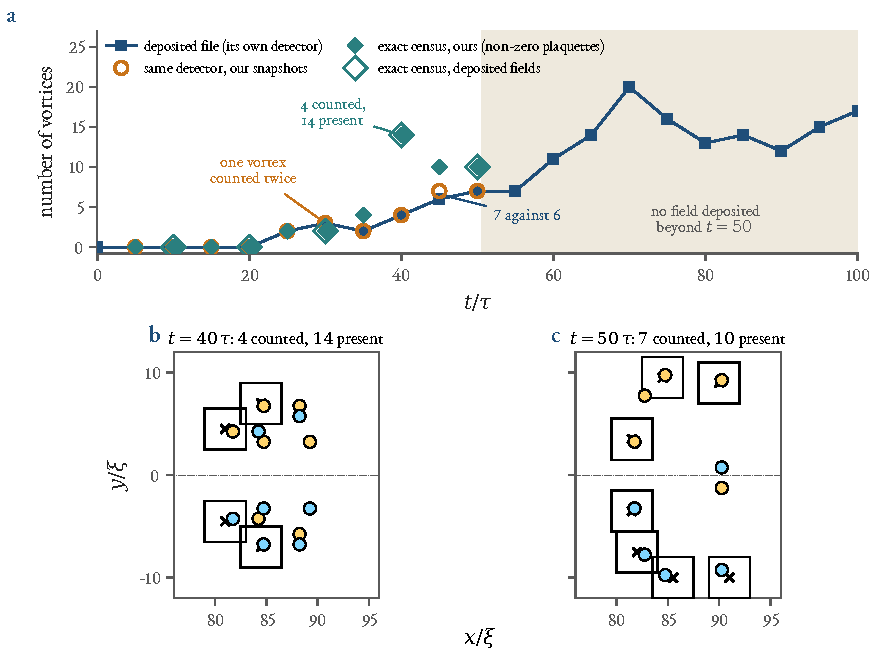
\includegraphics[width=\linewidth]{figures/ch09_census.pdf}
\caption[How many vortices?]{How many vortices? \textbf{a}, counts against time: the deposited file (blue squares, to $t=100\,\tau$), the same detector on our snapshots (open orange circles), and the exact census of non-zero plaquettes (teal diamonds: ours, filled; deposited fields, open). \textbf{b}, \textbf{c}, the deposited field at $t=40$ and $50\,\tau$: the plaquettes of non-zero winding (gold counter-clockwise, cyan clockwise) and, as black squares and crosses, the loops and centres of the detector's accepted vortices. Script \texttt{figures/ch09\_census.py}.}\label{ch09:fig-census}
\end{figure}

\paragraph{A fragile decision.} The detector's loop integral is not quantised, because it drops the large steps, and its decision is fragile. For the same vortex, the integral in the deposited field and in ours differs by up to $\cnineLoopDiffMax\,\pi$ (by $\cnineLoopDiffThirty\,\pi$ at $t=30$), against a threshold of $0.9\pi$, although the two fields agree to better than $\cninePsiFifty$ in relative $L^2$. At $t=45$, the one time at which the counts differ, no deposited field exists, so the vortex that the deposited detector missed cannot be identified. In our field the seven accepted vortices have loop integrals of $1.26\pi$ or more, except one, at $(x,y)=(\cnineMarginalX,-\cnineMarginalY)$, with $\cnineMarginalInt\,\pi$, which is $\cnineMarginalAbove\,\%$ above the threshold. It is the only candidate for which a perturbation of the size seen between the two runs at other times could flip the decision. That is a plausible explanation of the unit difference. It is not a demonstration.

\paragraph{Mirror symmetry.} The exact census is a set of mirror pairs: for each plaquette of charge $q$ at $(x,y)$ there is one of charge $-q$ at $(x,-y)$, in every snapshot of ours and in the deposited fields at $t=30$ and $40$; at $t=50$ the two plaquettes of the deposited field nearest to the axis have their partners one cell away. The relative $L^2$ distance of $\psi$ from its mirror image $\psi(x,-y)$ is $\cnineAsymZero$ at $t=0$ (the seeded noise), $\cnineAsymRefTen$ and $\cnineAsymOursTen$ at $t=10$ in the deposited field and in ours, and $\cnineAsymRefFifty$ and $\cnineAsymOursFifty$ at $t=50$: it decays instead of growing. Up to $t=50$ the flow is mirror-symmetric, and so, as far as the lift shows, is the deposited run up to $t=100$ (\cref{ch09:fig-force}\textbf{c}: the lift never exceeds $\cnineLiftRatio$ of the drag).

\section{The birth of a pair}\label{ch09:birth}

\paragraph{Zooming in time.} The snapshots are five time units apart; the first pair appears between two of them. To see it we continued our field from $t=20$ to $t=25$ with the same scheme in numpy (\texttt{figures/ch09\_birth\_run.py}), storing a $60\,\xi\times50\,\xi$ sub-box every $0.1\,\tau$. The continuation reproduces our Rust snapshot at $t=25$ to a relative $L^2$ distance of $\cnineContRel$: two implementations of one scheme, as they should be. \Cref{ch09:fig-birth} shows what happens.

\begin{figure}[t]\centering
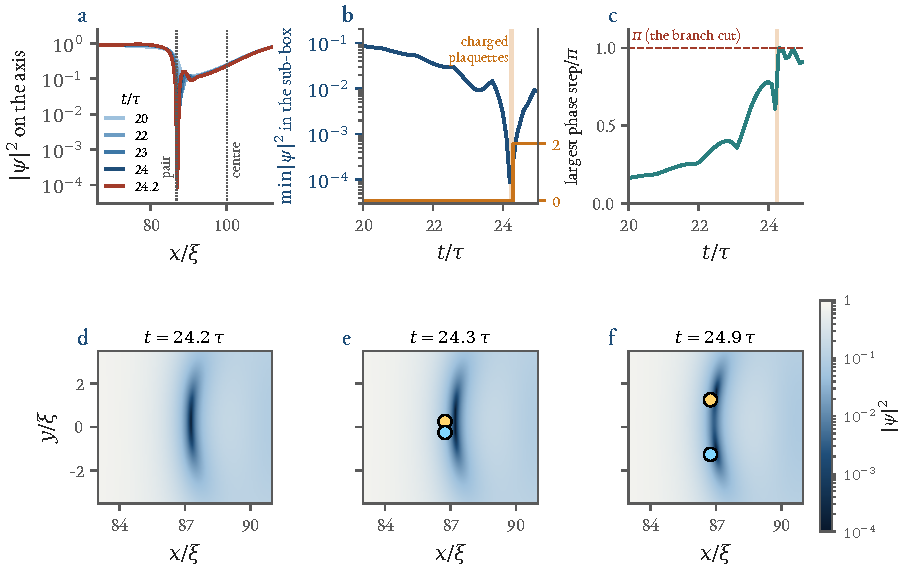
\includegraphics[width=\linewidth]{figures/ch09_birth.pdf}
\caption[The first vortex pair]{The first vortex pair, from the $0.1\,\tau$ continuation of our field. \textbf{a}, the density on the axis $y=0$ at five times; the dotted lines mark the birth site and the centre of the obstacle. \textbf{b}, the smallest density of the sub-box (blue, logarithmic) and the number of plaquettes of non-zero winding (orange); the shaded band is the interval in which the pair is born. \textbf{c}, the largest principal phase step on any edge of the sub-box, in units of $\pi$. \textbf{d}--\textbf{f}, the density (logarithmic colour scale, cubic interpolation) just before the birth, just after it and $0.6\,\tau$ later, with the charged plaquettes (gold counter-clockwise, cyan clockwise). Script \texttt{figures/ch09\_birth.py}.}\label{ch09:fig-birth}
\end{figure}

\paragraph{What happens.} On the axis the density minimum of the sub-box falls from $\cnineNminTwenty$ at $t=20$ to $\cnineNminTwentyThree$ at $t=23.3$, where it hesitates, and then, within a time unit, to $\cnineBirthNmin$ at $t=\cnineBirthBefore$. At $t=\cnineBirthAfter$ two plaquettes carry the charges $\mp1$, at $(x,y)=(\cnineBirthX,\mp\cnineBirthY)$: a vortex and an antivortex, $\cnineBirthSep\,\xi$ apart, on the axis, $\cnineBirthDist\,\xi$ downstream of the centre of the obstacle. Since the flow is mirror-symmetric a single pair has to be born on the axis, and it is. By $t=24.9$ the two are $\cnineBirthSepLate\,\xi$ apart. The pair appears at the downstream end of the supersonic region, which at $t=\cnineBirthAfter$ runs on the axis from $x=\cnineBirthSupLo$ to $\cnineBirthSupHi$: within a healing length of its edge.

\paragraph{Lean's edge case in the data.} The largest principal phase step on any edge of the sub-box is $\cnineEdgeTwentyFour\,\pi$ at $t=24.0$, $\cnineEdgeTwentyFourTwo\,\pi$ at $t=\cnineBirthBefore$ and $\cnineBirthEdge\,\pi$ at $t=\cnineBirthAfter$, the first time the pair exists (\cref{ch09:fig-birth}\textbf{c}). Two vortices of opposite sign one grid cell apart are the configuration in which the phase differs by almost $\pi$ across the edge that joins them. The branch cut that \Lthm{VortexWinding}{pdiff_add_rev_eq_two_pi_iff} isolates is therefore not a remote possibility: when the pair is born the largest step is within $0.2\,\%$ of $\pi$. No edge is exactly at $\pi$, so the census is an exact integer count of the sampled field. What that count means \emph{at birth} is not decided by the theorem. A pair half a healing length apart, on a grid whose spacing is half a healing length, is at the limit of what the sampled field resolves; resolution, not the theorem, decides whether the two plaquettes are two vortices of the continuum field.

\paragraph{Hydrodynamics on the data.} The reading of the run in terms of Bernoulli's relation and the supersonic region (\cref{ch09:landau}) rests on the Madelung form of \eqref{ch09:eq-model}. Write $\psi=\sqrt n\,\mathrm e^{\mathrm i\theta}$, $\mathbf u=\nabla\theta-v\,\mathbf e_x$ and $Q=-\nabla^2\!\sqrt n/(2\sqrt n)$, the quantum pressure. Where $\Gamma=0$, the phase obeys
\begin{equation}\label{ch09:eq-madelung}
-\partial_t\theta\;=\;R\;:=\;\tfrac12|\mathbf u|^2+n+V+Q-1-\tfrac12v^2 .
\end{equation}
For a stationary flow $R=0$: that is Bernoulli's relation with the quantum pressure restored. The algebraic part of the Madelung transformation, the splitting of the kinetic energy density into a quantum-pressure part and a hydrodynamic part, is a theorem of the library (\Lthm{MadelungSplit}{kinetic_density_split}); the dynamical identity \eqref{ch09:eq-madelung} is not, and we check it on the data. At $t=20.1$ we compute $R$ from a single snapshot of the sub-box (fourth-order differences) and $\partial_t\theta$ from the snapshots at $t=20.0$ and $20.2$. They agree: the correlation is $\cnineBernCorr$ ($1-r=\cnineBernOneMinus$), and the largest difference is $\cnineBernMaxDiff$ against an rms of $\cnineBernRms$ for $R$. The model, its signs, the quantum pressure and the differences are consistent.

The same quantity says how far the flow is from the stationary state that the one-dimensional theorem assumes. On the axis $R$ runs from $\cnineBernRlo$ to $\cnineBernRhi$, as large as the terms it balances: the phase is not stationary, and different points of the axis advance in phase at rates that differ by up to $\cnineBernRspan\,\mu/\hbar$. This is the phase accumulation across the obstacle that Kwon and Shin describe as the precursor of the phase slip that nucleates dipoles. The quantum pressure is small along most of the axis ($|Q|\le\cnineBernQsmall$ for $x<84$ or $x>92$) and large in the hole: $Q=\cnineBernQmin$ at $x=\cnineBernQx$. That is the quantitative content of the remark of the paper quoted in \cref{ch09:landau}, that the quantum pressure plays a crucial role in triggering shedding.

\section{What does not agree, and what we do not know}\label{ch09:gaps}

\paragraph{The plateau of the force difference.} The deposited force and ours separate from $t\approx\cnineZeroCross$. The difference $\Delta F=F_{\rm ours}-F_{\rm ref}$ changes sign there, reaches $\cninedFatFourteen$ at $t=14$, $\cninedFatTwenty$ at $t=20$ and $\cninedFatTwentyFour$ at $t=24$, when the first pair is born and the difference has reached $\cninePlateauFracAtBirth\,\%$ of its final value, and stays between $\cninePlateauMin$ and $\cninePlateauMax$ for $t\ge26$ (\cref{ch09:fig-force}\textbf{b}). Our drag is weaker than the deposited one by $\cnineForceOverallPct\,\%$ of the maximum force. Four things about this difference can be said, and none of them is a cause.
\begin{itemize}
\item It starts more than thirteen time units \emph{before} any vortex exists. The programme's design note on the external reproduction reads it as the signature of a perturbation amplified by the unstable wake, and the software paper \cite{Callens2026sw} says that the force separates ``once the wake exists''. What exists at $t=11$ is the supersonic region and the rarefaction behind it, not vortices; the first pair arrives when the difference has already grown to $\cninePlateauFracAtBirth\,\%$ of its final value. That reading is not supported and is corrected here.
\item It is smooth and does not oscillate. A constant delay between the two runs does not describe it: fitting $\Delta F=-\delta\,F_{\rm ref}'(t)$ window by window gives $\delta=\cnineShiftTwenty$, $\cnineShiftThirty$ and $\cnineShiftForty\,\tau$ for the windows $20$--$30$, $30$--$40$ and $40$--$50$, with residuals of $\cnineShiftResTwenty\,\%$, $\cnineShiftResThirty\,\%$ and $\cnineShiftResForty\,\%$ of the difference: a delay would be one number with small residuals.
\item The mirror-symmetry-breaking channel is not what grows. The lift of the deposited run stays at $\cnineLiftRatio$ of the drag up to $t=100$, our lift at the snapshot times agrees with it to $\cnineLiftRelMax\,\%$, and the asymmetry of both fields decays (\cref{ch09:count}).
\item The fields differ everywhere, mildly: the rms density difference is between $\cnineDensRmsMin$ and $\cnineDensRmsMax$ at all five times, and the part of its square sum that lies within $40\,\xi$ of the obstacle (about $4\,\%$ of the area of the box) is $\cnineNearShareTen\,\%$ at $t=10$, $\cnineNearShareTwenty\,\%$ at $t=20$, and then $\cnineNearShareThirty$, $\cnineNearShareForty$ and $\cnineNearShareFifty\,\%$ as the vortices form. The relative $L^2$ distance of $\psi$ itself, $\cninePsiFifty$ at $t=50$, drops only to $\cninePsiGaugeFifty$ when a global phase (a gauge, $\cnineGlobalPhaseFifty$ at that time) is removed.
\end{itemize}
The force is a delicate functional. It weighs the density by $\partial_xV$, which is odd about the centre of the obstacle and has the maximum modulus $(2/\sigma)V_0\mathrm e^{-1/2}=0.055$ per healing length; a coherent density difference of a few $10^{-4}$ over the region where $\partial_xV$ is large is enough to move it by $10^{-2}$.

\paragraph{Candidate causes, none tested.} Three differences between the two computations could produce a smooth, slowly growing difference of this size. The reference works in single precision. Its splitting is of second order with $\Delta t=0.01$, while our scheme has a temporal error of $\cnineOwnTemporal$ in the force at $t\le5$ (\cref{ch09:repro}). And the local step of its code integrates the damping exactly only where $\Gamma>0.01$ and treats the rest of the box as unitary, while its linear step uses the full $\Gamma$. Our scheme has none of the three. The first two are properties of the reference's arithmetic and discretisation; the third is a difference between what the code does and the model \eqref{ch09:eq-model} that we recovered from it, and would be a defect of our recovery rather than of the reference. What would settle it is a numpy port of the reference's own stepper, run in double and in single precision from the deposited field: the first run would separate the splitting from the arithmetic. We did not do it.

\paragraph{What was not done.} The deposited force and counts go on to $t=100$; our run stops at $t=50$, where the deposited snapshots stop, and a longer Rust run costs $\cnineProdWallMin$ minutes of wall-clock time per fifty time units on the shared machine. After $t=50$ the deposited detector's count rises to $20$ at $t=70$ and then fluctuates between $12$ and $17$. Nothing in the first hundred time units shows the alternating same-sign clusters that the paper describes at this velocity; they belong to its averaging window of $\cninePaperTLo$ to $\cninePaperTHi\,\tau$, and the lift is still $\cnineLiftRatio$ of the drag. We computed no Strouhal number, drag coefficient, Reynolds number or effective diameter. The width of the supersonic region at $t=20$, $\cnineSupWidthOursTwenty\,\xi$, is an \emph{instantaneous} quantity of a region that has not yet shed a vortex; it is not the paper's time-averaged $D_{\rm eff}$ and must not be compared with it. Our run has no vortex removal near the boundary, as the paper's has; the deposited log records that the code's routine removed none in the first $100\,\tau$ (the two count columns of its file are equal). There is no GPU on this machine, and no comparison with the authors' code was possible beyond its deposited output.

\begin{honestbox}
\textbf{Proved} (Lean 4, kernel-checked, standard axioms only): that the Landau velocity of the uniform Gross--Pitaevskii dispersion is exactly the speed of sound; that a flow is locally supersonic iff $n^3<j^2$, and, with Bernoulli's relation, iff $u^2>\tfrac23(B-V)$; that Bernoulli's function at fixed flux is minimised at the sonic point and that this bounds the height of a barrier that a steady channel flow can cross; that holding a linear ramp at the end of each step overshoots its integral by $ah^2n/2$; that the principal-difference winding around a closed loop is an integer multiple of $2\pi$. These are theorems about numbers and finite sums. They say nothing about the Gross--Pitaevskii dynamics. The library's Landau lemmas formalise a paragraph of the review of Godfrin and Krotscheck as inequalities between numbers, not as statements about a measured curve.\par
\textbf{Simulated and compared} (Rust, double precision, against a deposited single-precision run): the force on the obstacle to $\cnineForceTen$ for $t\le10$ and to $\cnineForceOverallPct\,\%$ of its maximum for $t\le50$; $\psi$ to $\cninePsiFifty$ at $t=50$; the position and sign of $\cnineMatchTotal$ vortices, $\cnineMatchTotalIdent$ of them on the same plaquette; the area of the supersonic region at $t=20$ to $0.4\,\%$. Nothing here is a laboratory measurement, and nothing is a reproduction of the paper's results.\par
\textbf{Only an analogy}: the one-dimensional choked flow as a picture of the two-dimensional threshold. Its premise, a flux conserved along the channel, fails in the data (the flux at the centre of the obstacle is $\cnineAxisJratio\,\%$ of the upstream flux), and it puts the threshold a factor ten below the paper's; the ramp theorem's resemblance to the library's calibration lemmas is a resemblance of method.\par
\textbf{Failed or unresolved}: the registered tolerance $10^{-5}$ for the force at $t\le10$ is not met ($\cnineForceRelTen$); the cause of the force difference of $\cnineForceOverallPct\,\%$ is not identified, and the earlier explanation of it is withdrawn; the single difference of the detector's counts at $t=45$ is explained only as plausible; nothing was run beyond $t=50$.
\end{honestbox}

\section{Exercises}\label{ch09:exercises}

\paragraph{Exercise 1.} Prove \lean{bernoulli\_min} by hand, and then \lean{barrier\_height\_bound}. Show that $V_c(s)=(1-s)^2(s+2)/2$ decreases on $(0,1)$ and that $V_c\approx\tfrac32(1-s)^2$ near $s=1$, hence $V_c\approx\tfrac23(1-j)^2$ near $j=1$; compare with the exact value $\cnineVc$ at $j=0.55$ (the approximation gives $\cnineVcApprox$). In two sentences, say why a weak barrier does not choke a flow with $j<1$ although for $j=1$ every barrier does. \emph{Hint:} the factorisation $2n^3-3sn^2+s^3=(n-s)^2(2n+s)$; for the last part, what is $V_c(1)$?

\paragraph{Exercise 2.} Load \texttt{psi\_time\_50.0.npy} of the archive, compute the exact census with the functions of \cref{ch09:count}, and check that it contains ten plaquettes. Then apply the detector's merging rule, dropping every vortex within $3\,\xi$ of an earlier one, to the census. How many vortices remain at $t=40$ and at $t=50$, and how does the answer depend on the merging radius? Does any radius make the census reproduce the detector's counts $4$ and $7$? \emph{Hint:} \texttt{scipy.spatial.cKDTree}; the detector also requires a density minimum below $0.2$ along the first array axis, which a census does not.

\paragraph{Exercise 3.} Suppose the reference had read the velocity at the \emph{start} of each step. State the analogue of \lean{ramp\_overshoot} (the sum over $i=0,\dots,n-1$ of $a(ih)h$) and prove it, in Lean or by induction. Using the sensitivity of the force to a displacement of the obstacle, $\cnineSensA\,\mu/\xi^2$, predict the sign and size of the difference between our stage-time run and that hypothetical reference at $t=0.1$, and the difference between that reference and the actual one. \emph{Hint:} the displacement error is now an undershoot of the same size; the answer for the first is a difference of the size of the offset of \cref{ch09:repro} and of opposite sign, and the second is twice as large.

\section{Notes and further reading}\label{ch09:notes}

The reproduced run, and all that is quoted of its paper, is that of Kwon and Shin \cite{KwonShin2026prr}, whose open archive \cite{KwonShin2026data} (MIT for the code, CC BY 4.0 for the processed data, as its README says) makes a reproduction of this kind possible at all. For the local criterion that organises their analysis, the early studies are the numerical discovery of vortex emission in the Gross--Pitaevskii model by Frisch, Pomeau and Rica \cite{FrischPomeauRica1992}, and its analysis near the transonic transition by Josserand, Pomeau and Rica \cite{JosserandPomeauRica1999}; Winiecki and collaborators studied vortex shedding and drag in dilute condensates \cite{Winiecki2000}, and the superfluid Reynolds number that the paper adapts to penetrable obstacles comes from Reeves, Billam, Anderson and Bradley \cite{Reeves2015}. The critical velocity of a Gaussian obstacle is the subject of Kwak, Jung and Shin \cite{Kwak2023}, and the laboratory experiments mentioned at the start are \cite{Raman1999,Kwon2015PRA,Kwon2016PRL}. Landau's argument is in \cite{Landau1941}; the statement of it that the Lean library formalises is the paragraph of the review of Godfrin and Krotscheck \cite{GodfrinKrotscheck2022}, and the spectrum that enters it, for helium, is the one measured by Godfrin and co-workers \cite{Godfrin2021}. Pitaevskii and Stringari \cite{PitaevskiiStringari2016} and Donnelly \cite{Donnelly1991} cover the hydrodynamics and the vortices. The engine, its verification and the reproduction are those of the software paper \cite{Callens2026sw}; the library is \cite{Callens2026lib}; the comparison records are in \texttt{docs/designs/PGPE\_EXTERNAL\_REPRODUCTION.md} of the repository and in the ledger entries CLAIM-103 and CLAIM-106. The next steps, in the order we would take them, are the numpy port of the reference's stepper to separate precision from splitting, a run of the Rust engine to $t=100$, and a long run of the Rust engine at the deposited parameters, over the paper's window of $\cninePaperTLo\,\tau$ and more, from which the paper's time-averaged supersonic region and its $D_{\rm eff}$ could be computed.
